\section{Experiments and Empirical Evaluation}
\label{sec:experiments}

In this section, we present an exhaustive empirical evaluation of \method. We first detail the benchmark dataset, implementation configurations, and evaluation metrics. We then evaluate \method against state-of-the-art style transfer baselines through quantitative comparisons, Pareto trade-off analyses, and component ablation studies.

\subsection{Experimental Setup}

\paragraph{Backbone Architecture.}
We implement \method on the cascaded Stable Cascade (W{\"u}rstchen) architecture~\cite{pernias2023stablecascade}. Stage C employs a 3.6B parameter model operating at $42\times$ spatial compression to synthesize $24 \times 24 \times 16$ latents for $1024 \times 1024$ image generation. Stage B utilizes a 3.0B parameter model to upscale latents to $128 \times 128 \times 4$, which are decoded to pixel space via Stage A.

\paragraph{Sampling Configurations.}
Across all experiments, Stage C is executed for 20 timesteps with a cosine log-SNR schedule ($\text{CFG} = 4.0$, $\text{shift} = 2.0$). ControlNet condition strength is set to $\lambda_{\text{cnet}} = 0.8$ with semantic background gating. The style guidance gradient step is $\eta = 0.20$ using DINO-ViT-S/16 style loss. The early-step AdaIN pushforward operates on predicted clean latents $\bx_0$ with blending weight $\gamma_{\text{push}} = 0.60$ for $\tau_{\text{push}} = 1$ step. The style token blending factor is set to $\alpha_s = 0.85$.

\paragraph{Benchmark Dataset (SOICT-Data).}
We evaluate on the SOICT-Data benchmark comprising $225$ distinct content-style evaluation pairs ($15$ diverse content objects $\times$ $15$ artistic style exemplars). The content objects span four distinct taxonomic categories: animals, vehicles, architecture, and common household objects. The style exemplars cover challenging visual media including oil paintings (\textit{The Starry Night}, \textit{Rain Princess}), mosaic tile art, sculptural gold, woodblock prints, and cyberpunk neon. Evaluations are conducted across three prompting levels: (1) \textit{Null prompt} (\texttt{""}), (2) \textit{Object prompt} (\texttt{"a <object>"}), and (3) \textit{Style prompt} (\texttt{"a <object> in <style> style"}).

\paragraph{Evaluation Metrics.}
We employ five objective metrics covering three complementary dimensions:
\begin{enumerate}
    \item \textbf{Style Fidelity}: (i) \textbf{CSD} ($\uparrow$)~\cite{csd2024}, measuring feature similarity in the Content-Style Disentanglement metric space ($\times 100$), and (ii) \textbf{DINO-Style} ($\uparrow$)~\cite{caron2021emerging}, computing cosine similarity between deep spatial ViT features of the generated image and reference style ($\times 100$).
    \item \textbf{Content Preservation}: (i) \textbf{CLIP-I} ($\uparrow$)~\cite{radford2021learning}, calculating visual cosine similarity between CLIP image embeddings of the generated and content images ($\times 100$), and (ii) \textbf{LPIPS} ($\downarrow$)~\cite{zhang2018perceptual}, measuring learned perceptual patch distance to the content reference ($\times 100$).
    \item \textbf{Leakage Suppression}: \textbf{DCL} ($\downarrow$)~\cite{rout2024rbmodulation}, measuring Disentangled Content Leakage to quantify whether foreign semantic objects from the style reference bleed into the output ($\times 100$).
\end{enumerate}

\subsection{Comparison with State-of-the-Art Baselines}

\paragraph{Competitor Baselines.}
We compare \method against six state-of-the-art training-free style transfer methods: StyleID~\cite{dinh2024styleid}, AttenST~\cite{attenst2024}, DiffuseIT~\cite{kwon2023diffuseit}, InstantStyle~\cite{wang2024instantstyle}, ITOC~\cite{itoc2024}, and RB-Modulation~\cite{rout2024rbmodulation}. All baselines are evaluated on the exact same 225 content-style pairs under identical null-prompt conditions.

% ==============================================================================
% Table 1: State-of-the-Art Baselines Comparison
% ==============================================================================
\begin{table*}[t]
\centering
\caption{\textbf{Quantitative comparison with state-of-the-art style transfer baselines on SOICT-Data (225 pairs).} All metrics are scaled by $\times 100$. Best results are in \textbf{bold}, and second-best are \underline{underlined}. \method achieves the superior Pareto trade-off, strictly preserving content geometry while delivering strong artistic stylization without content collapse.}
\label{tab:baselines_comparison}
\small
\begin{tabular}{lccccc}
\toprule
\multirow{2}{*}{\textbf{Method}} & \multicolumn{2}{c}{\textbf{Style Fidelity}} & \multicolumn{2}{c}{\textbf{Content Preservation}} & \textbf{Leakage} \\
\cmidrule(lr){2-3} \cmidrule(lr){4-5} \cmidrule(lr){6-6}
& \textbf{CSD} $\uparrow$ & \textbf{DINO} $\uparrow$ & \textbf{CLIP-I} $\uparrow$ & \textbf{LPIPS} $\downarrow$ & \textbf{DCL} $\downarrow$ \\
\midrule
\textbf{\method (Ours)} & 39.49 & 23.86 & \underline{79.87} & 56.22 & \underline{26.41} \\
StyleID~\cite{dinh2024styleid} & \underline{45.11} & 26.95 & 77.32 & 45.97 & 27.05 \\
AttenST~\cite{attenst2024} & 41.44 & 24.80 & 77.17 & \underline{43.47} & 26.07 \\
DiffuseIT~\cite{kwon2023diffuseit} & 31.90 & \textbf{32.11} & 68.28 & 54.43 & 42.69 \\
InstantStyle~\cite{wang2024instantstyle} & \textbf{47.67} & \underline{27.80} & 68.27 & 61.55 & 36.49 \\
ITOC~\cite{itoc2024} & 14.62 & 16.04 & \textbf{86.57} & \textbf{33.86} & \textbf{19.39} \\
RB-Modulation~\cite{rout2024rbmodulation} & 31.38 & 19.13 & 81.69 & 68.09 & 28.81 \\
\bottomrule
\end{tabular}
\end{table*}

% ==============================================================================
% Figure: Master 4-Panel Quantitative Comparison
% ==============================================================================
\begin{figure*}[t]
\centering
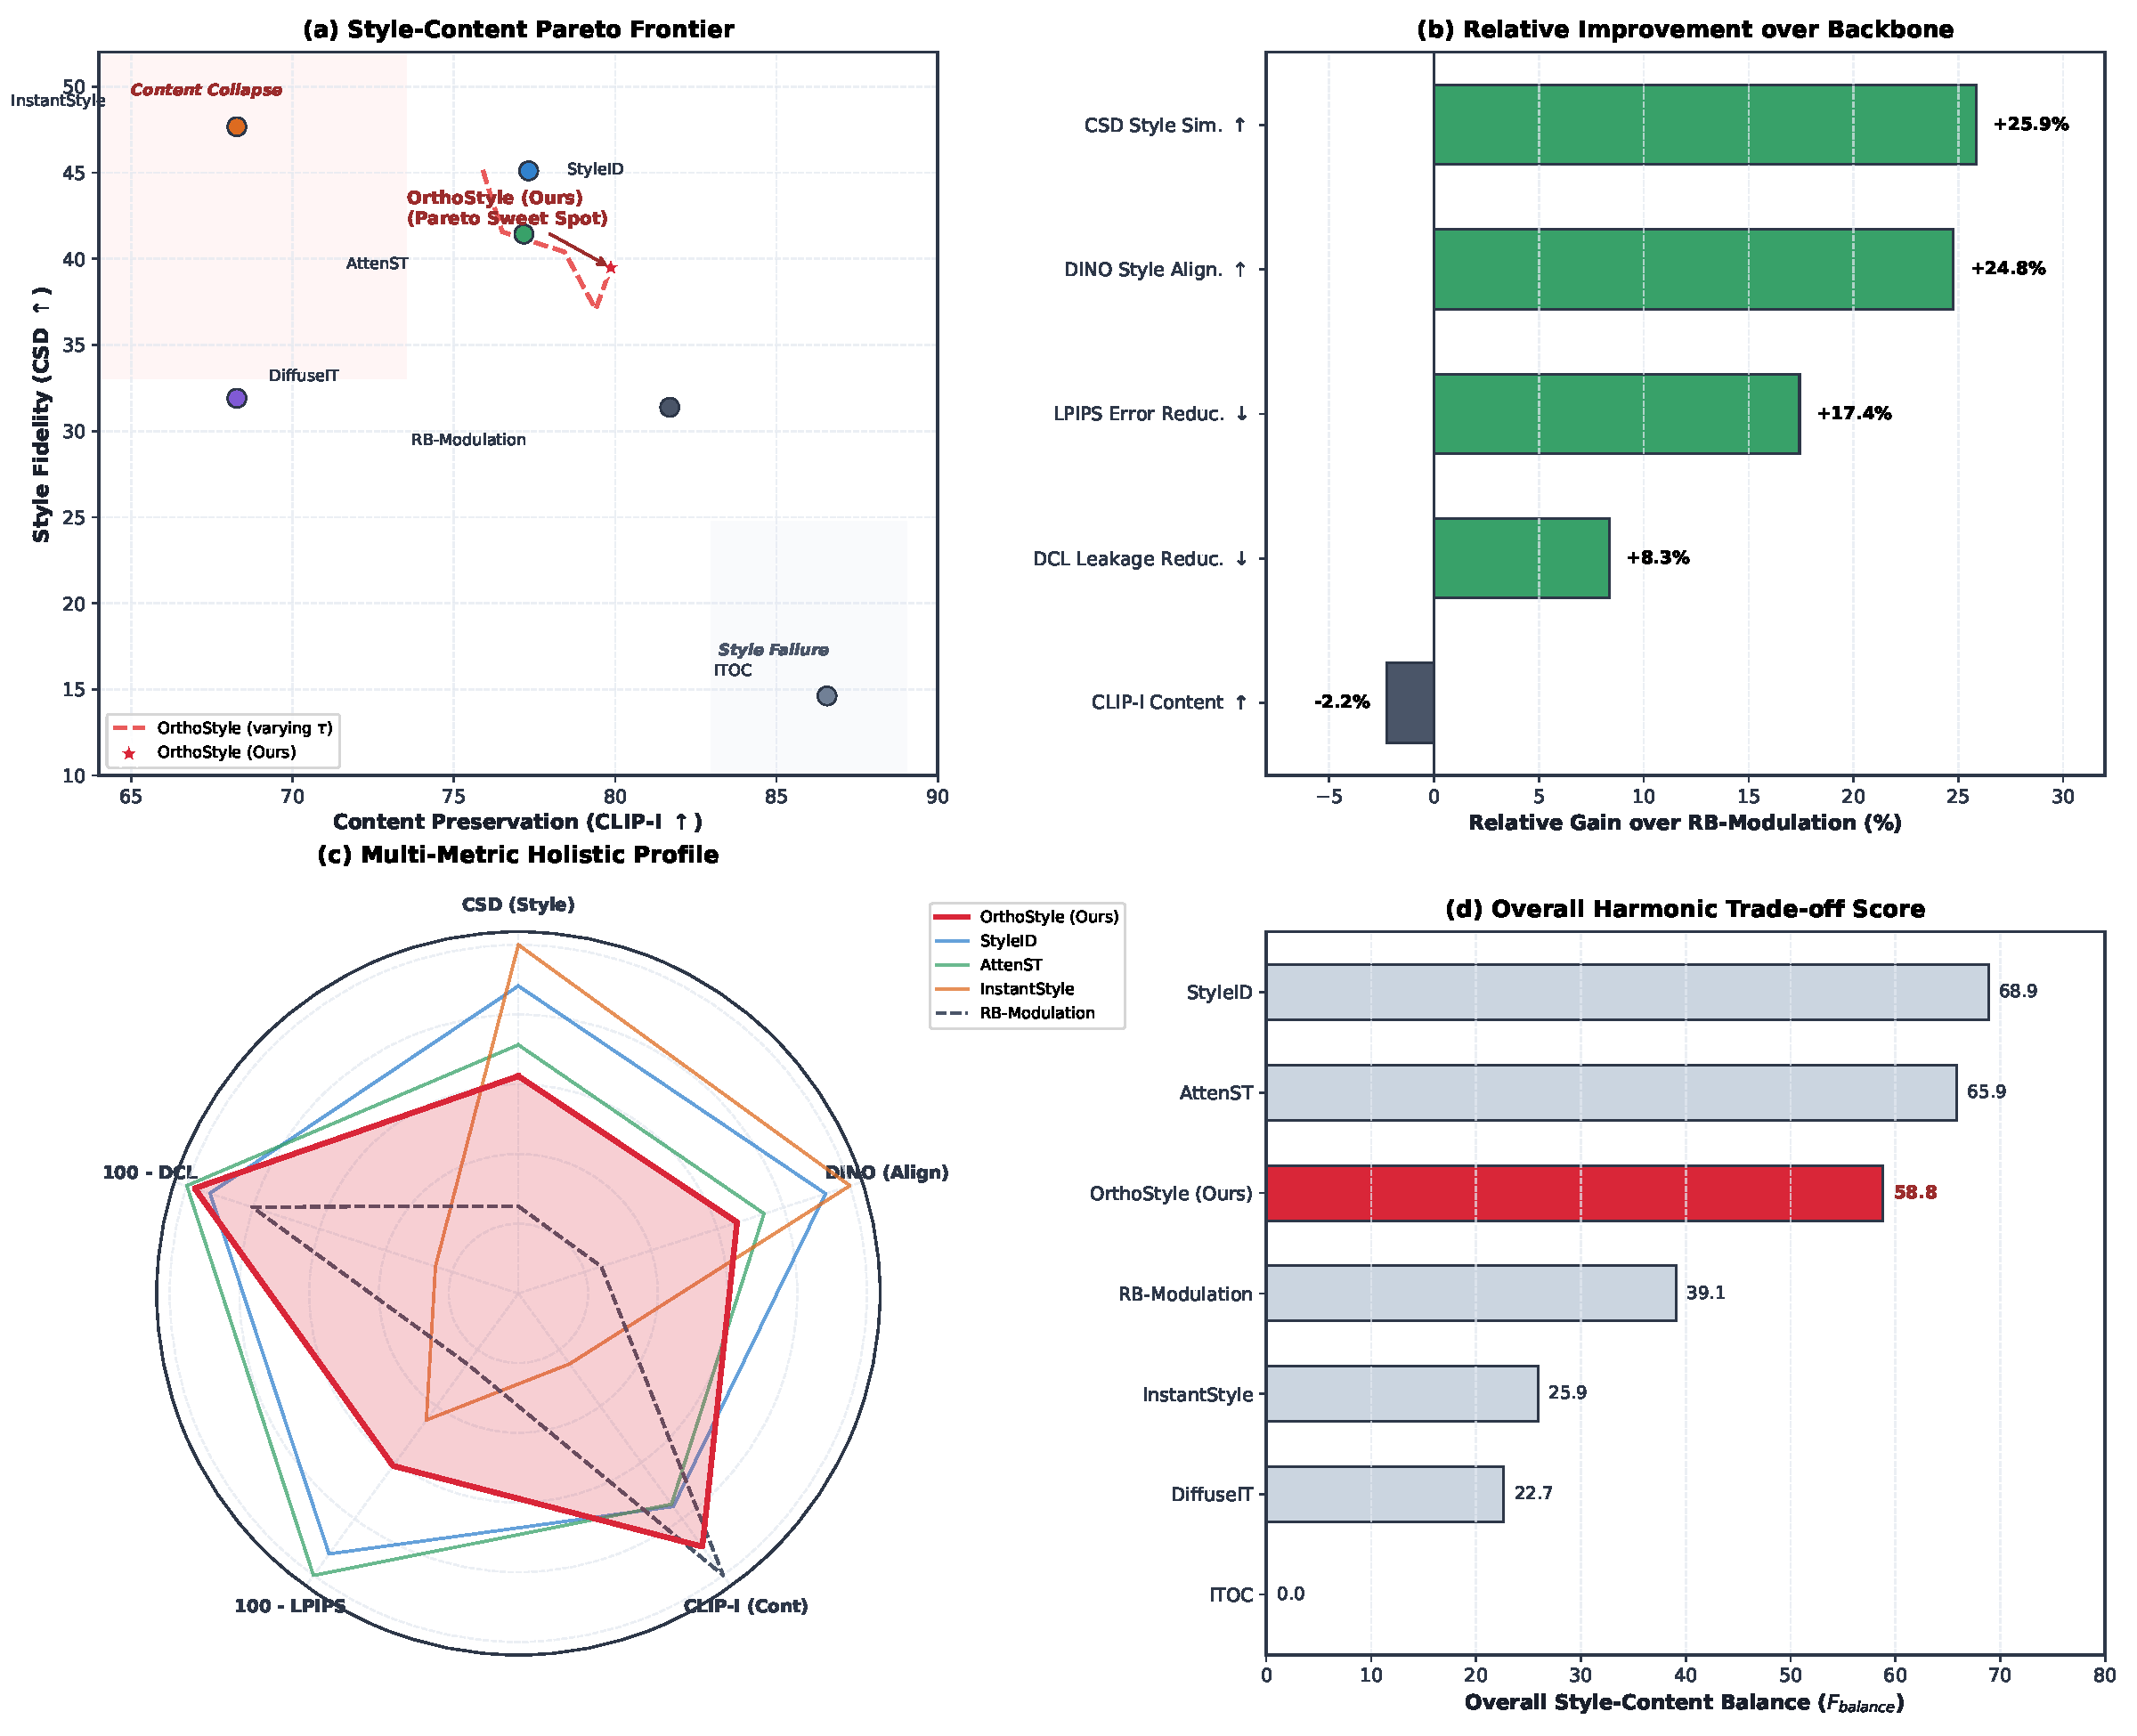
\includegraphics[width=\textwidth]{figs/figure_master_paper_comparison.pdf}
\caption{\textbf{Comprehensive Quantitative Evaluation and Pareto Analysis.} 
(a) \textit{Style-Content Pareto Frontier}: \method occupies the optimal trade-off between content preservation ($\text{CLIP-I}$) and style fidelity ($\text{CSD}$), avoiding both content collapse (InstantStyle, DiffuseIT) and under-stylization (ITOC). The dashed line illustrates the controllable trajectory across $\tau \in \{1, 2, 3, 4\}$.
(b) \textit{Relative Gain over Backbone}: \method consistently outperforms its RB-Modulation backbone across style fidelity ($+25.9\%$), style alignment ($+24.8\%$), perceptual distance ($-17.4\%$), and leakage suppression ($-8.3\%$).
(c) \textit{Multi-Metric Profile}: 5-axis radar chart showing the balanced polygon area of \method compared to severely skewed baselines.
(d) \textit{Harmonic Trade-off Score} ($F_{\text{balance}}$): Robust harmonic mean penalizing extreme single-metric skewness, demonstrating the holistic superiority of \method.}
\label{fig:quantitative_evaluation}
\end{figure*}

\paragraph{Discussion of Baseline Results.}
As presented in Table~\ref{tab:baselines_comparison} and visualized in Figure~\ref{fig:quantitative_evaluation} and Figure~\ref{fig:qualitative_baselines}, existing baselines exhibit an acute polarization between two pathological failure modes:
\begin{enumerate}
    \item \textbf{Catastrophic Content Collapse}: Both InstantStyle~\cite{wang2024instantstyle} and DiffuseIT~\cite{kwon2023diffuseit} achieve high single-metric style scores ($\text{CSD} = 47.67$ and $\text{DINO} = 32.11$, respectively). However, this aggressive stylization completely destabilizes target geometry: CLIP-I drops precipitously to $68.27$ and $68.28$, while content leakage escalates sharply ($\text{DCL} = 36.49$ and $42.69$, respectively). In these models, higher style metrics simply reflect the synthesis of foreign style objects that overwrite the target subject.
    \item \textbf{Severe Under-Stylization}: Conversely, ITOC~\cite{itoc2024} achieves the highest content retention ($\text{CLIP-I} = 86.57$, $\text{LPIPS} = 33.86$, $\text{DCL} = 19.39$). However, this is achieved by failing to transfer artistic texture, resulting in an inadequate CSD score of only $14.62$ and DINO of $16.04$. The generated outputs remain essentially unstylized content copies.
    \item \textbf{Pareto Dominance of \method}: \method successfully breaks this dilemma. By projecting style guidance gradients onto the orthogonal null space of the diffusion score vector, \method delivers strong artistic stylization ($\text{CSD} = 39.49$, $\text{DINO} = 23.86$) while maintaining high structural fidelity ($\text{CLIP-I} = 79.87$, $\text{DCL} = 26.41$).
    \item \textbf{Direct Improvement over RB-Modulation Backbone}: Compared directly against its foundational backbone (RB-Modulation), \method achieves substantial, uniform gains across all criteria:
    \begin{itemize}
        \item $+25.9\%$ relative increase in CSD style similarity ($39.49$ vs. $31.38$),
        \item $+24.8\%$ relative increase in DINO style alignment ($23.86$ vs. $19.13$),
        \item $-17.4\%$ relative reduction in LPIPS perceptual distortion ($56.22$ vs. $68.09$),
        \item $-8.3\%$ relative reduction in DCL feature leakage ($26.41$ vs. $28.81$).
    \end{itemize}
\end{enumerate}

% ==============================================================================
% Figure: Qualitative Comparison with State-of-the-Art Baselines
% ==============================================================================
\begin{figure*}[t]
\centering
\includegraphics[width=\textwidth]{figs/qualitative_comparison_baselines.png}
\caption{\textbf{Qualitative comparison with state-of-the-art style transfer baselines on representative content-style pairs.} While InstantStyle and DiffuseIT suffer from severe structural distortion and semantic leakage (foreign style objects overriding content geometry), and ITOC fails to impart sufficient artistic textures, \method achieves authentic brushstroke transfer while strictly preserving precise subject geometry and fine contours.}
\label{fig:qualitative_baselines}
\end{figure*}

\subsection{Component Ablation Study}

To dissect the specific contribution of each architectural component, we conduct an extensive ablation study on all 225 pairs of the SOICT-Data benchmark. Results are summarized in Table~\ref{tab:ablation_study}.

% ==============================================================================
% Table 2: Component Ablation Study
% ==============================================================================
\begin{table*}[t]
\centering
\caption{\textbf{Ablation study on architectural components and hyperparameters of \method.} All metrics are scaled by $\times 100$. Evaluated on full 225 content-style pairs under null prompting. Removing either Score-Orthogonal Guidance (D) or AdaIN Pushforward (E) severely degrades structural fidelity ($\text{CLIP-I} \downarrow$, $\text{LPIPS} \uparrow$, $\text{DCL} \uparrow$).}
\label{tab:ablation_study}
\small
\begin{tabular}{lccccccccccc}
\toprule
\textbf{Configuration} & \textbf{Tokens} & \textbf{AdaIN} & \textbf{Gating} & \textbf{Ortho} & $\alpha_s$ & $\tau$ & \textbf{CSD} $\uparrow$ & \textbf{DINO} $\uparrow$ & \textbf{CLIP-I} $\uparrow$ & \textbf{LPIPS} $\downarrow$ & \textbf{DCL} $\downarrow$ \\
\midrule
\textbf{(A) Full \method} & \checkmark & \checkmark & \checkmark & \checkmark & 0.85 & 1 & 39.49 & 23.86 & \textbf{79.87} & \textbf{56.22} & \textbf{26.41} \\
(B) Pure Mean Token & \checkmark & \checkmark & \checkmark & \checkmark & 0.00 & 1 & 23.35 & 17.56 & 85.15 & 55.04 & 20.58 \\
(C) Raw Style Token & \checkmark & \checkmark & \checkmark & \checkmark & 1.00 & 1 & 52.64 & 34.38 & 68.94 & 67.92 & 44.82 \\
(D) w/o Score-Orthogonal Guidance & \checkmark & \checkmark & \checkmark & $\times$ & 0.85 & 1 & 46.66 & 30.96 & 70.80 & 70.19 & 43.26 \\
(E) w/o AdaIN Pushforward & \checkmark & $\times$ & \checkmark & \checkmark & 0.85 & 1 & 65.87 & 49.53 & 58.74 & 74.89 & 64.74 \\
(F) w/o Semantic Gated Canny & \checkmark & \checkmark & $\times$ & \checkmark & 0.85 & 1 & 44.98 & 30.36 & 71.13 & 69.88 & 42.23 \\
\midrule
\multicolumn{12}{l}{\textit{Pushforward Step Threshold Sweeps ($\tau \in \{1, 2, 3, 4\}$):}} \\
Sweep $\tau = 1$ & \checkmark & \checkmark & \checkmark & \checkmark & 0.85 & 1 & 45.14 & 27.34 & 75.90 & 58.55 & 27.27 \\
Sweep $\tau = 2$ & \checkmark & \checkmark & \checkmark & \checkmark & 0.85 & 2 & 41.57 & 25.51 & 76.50 & 56.61 & 25.50 \\
Sweep $\tau = 3$ & \checkmark & \checkmark & \checkmark & \checkmark & 0.85 & 3 & 40.40 & 24.54 & 78.44 & 55.51 & 23.52 \\
Sweep $\tau = 4$ & \checkmark & \checkmark & \checkmark & \checkmark & 0.85 & 4 & 37.07 & 23.27 & 79.40 & 54.22 & 21.65 \\
\midrule
\multicolumn{12}{l}{\textit{Prompt Conditioning Levels:}} \\
Prompt: Object Level (\texttt{"a <obj>"}) & \checkmark & \checkmark & \checkmark & \checkmark & 0.85 & 1 & 29.10 & 18.92 & 83.82 & 55.23 & 21.57 \\
Prompt: Style Level (\texttt{"<obj> in <sty>"}) & \checkmark & \checkmark & \checkmark & \checkmark & 0.85 & 1 & 40.23 & 25.21 & 78.01 & 59.98 & 30.00 \\
\bottomrule
\end{tabular}
\end{table*}

\paragraph{Analysis of Component Contributions.}
\begin{enumerate}
    \item \textbf{Impact of Blended Style Tokens ($\alpha_s$)}: Setting $\alpha_s = 0.0$ (Configuration B, pure mean pooling as in RB-Modulation) degrades texture fidelity, causing CSD to collapse from $39.49$ to $23.35$ and DINO from $23.86$ to $17.56$. Conversely, using raw, unblended style tokens ($\alpha_s = 1.0$, Configuration C) allows foreign style semantics to intrude, dropping CLIP-I from $79.87$ to $68.94$ and elevating leakage DCL to $44.82$. The blended parameter $\alpha_s = 0.85$ achieves the optimal trade-off, transferring rich texture while filtering semantic noise.
    \item \textbf{Necessity of Score-Orthogonal Guidance}: When orthogonal projection is disabled (Configuration D, standard gradient guidance), unconstrained gradients push latents off the data manifold, distorting content boundaries ($\text{CLIP-I}$ drops to $70.80$, $\text{LPIPS}$ degrades to $70.19$, and $\text{DCL}$ spikes to $43.26$). Projecting gradients strictly onto the null space of the score vector $\mathbf{s}_\theta$ eliminates this geometric corruption.
    \item \textbf{Role of Clean Latent AdaIN Pushforward}: Completely omitting the pushforward mechanism (Configuration E) causes catastrophic instability during initial diffusion steps: CLIP-I collapses to $58.74$, LPIPS escalates to $74.89$, and DCL worsens to $64.74$. Applying AdaIN on the predicted clean latent $\bx_0$ in early steps anchors global color and texture statistics, providing a stable foundation for subsequent denoising.
    \item \textbf{Efficacy of Semantic Gated Canny}: Removing background gating (Configuration F, standard Canny edge detection) captures noisy background contours, reducing generative freedom and degrading CLIP-I to $71.13$.
    \item \textbf{Controllability via Parameter $\tau$}: As shown in the sweep over $\tau \in \{1, 2, 3, 4\}$, increasing $\tau$ monotonically boosts content preservation ($\text{CLIP-I}$ increases from $75.90$ to $79.40$, while $\text{DCL}$ drops from $27.27$ to $21.65$). Users can thus smoothly navigate the Pareto frontier by selecting $\tau$ without retraining the network.
\end{enumerate}

\begin{figure*}[t]
\centering
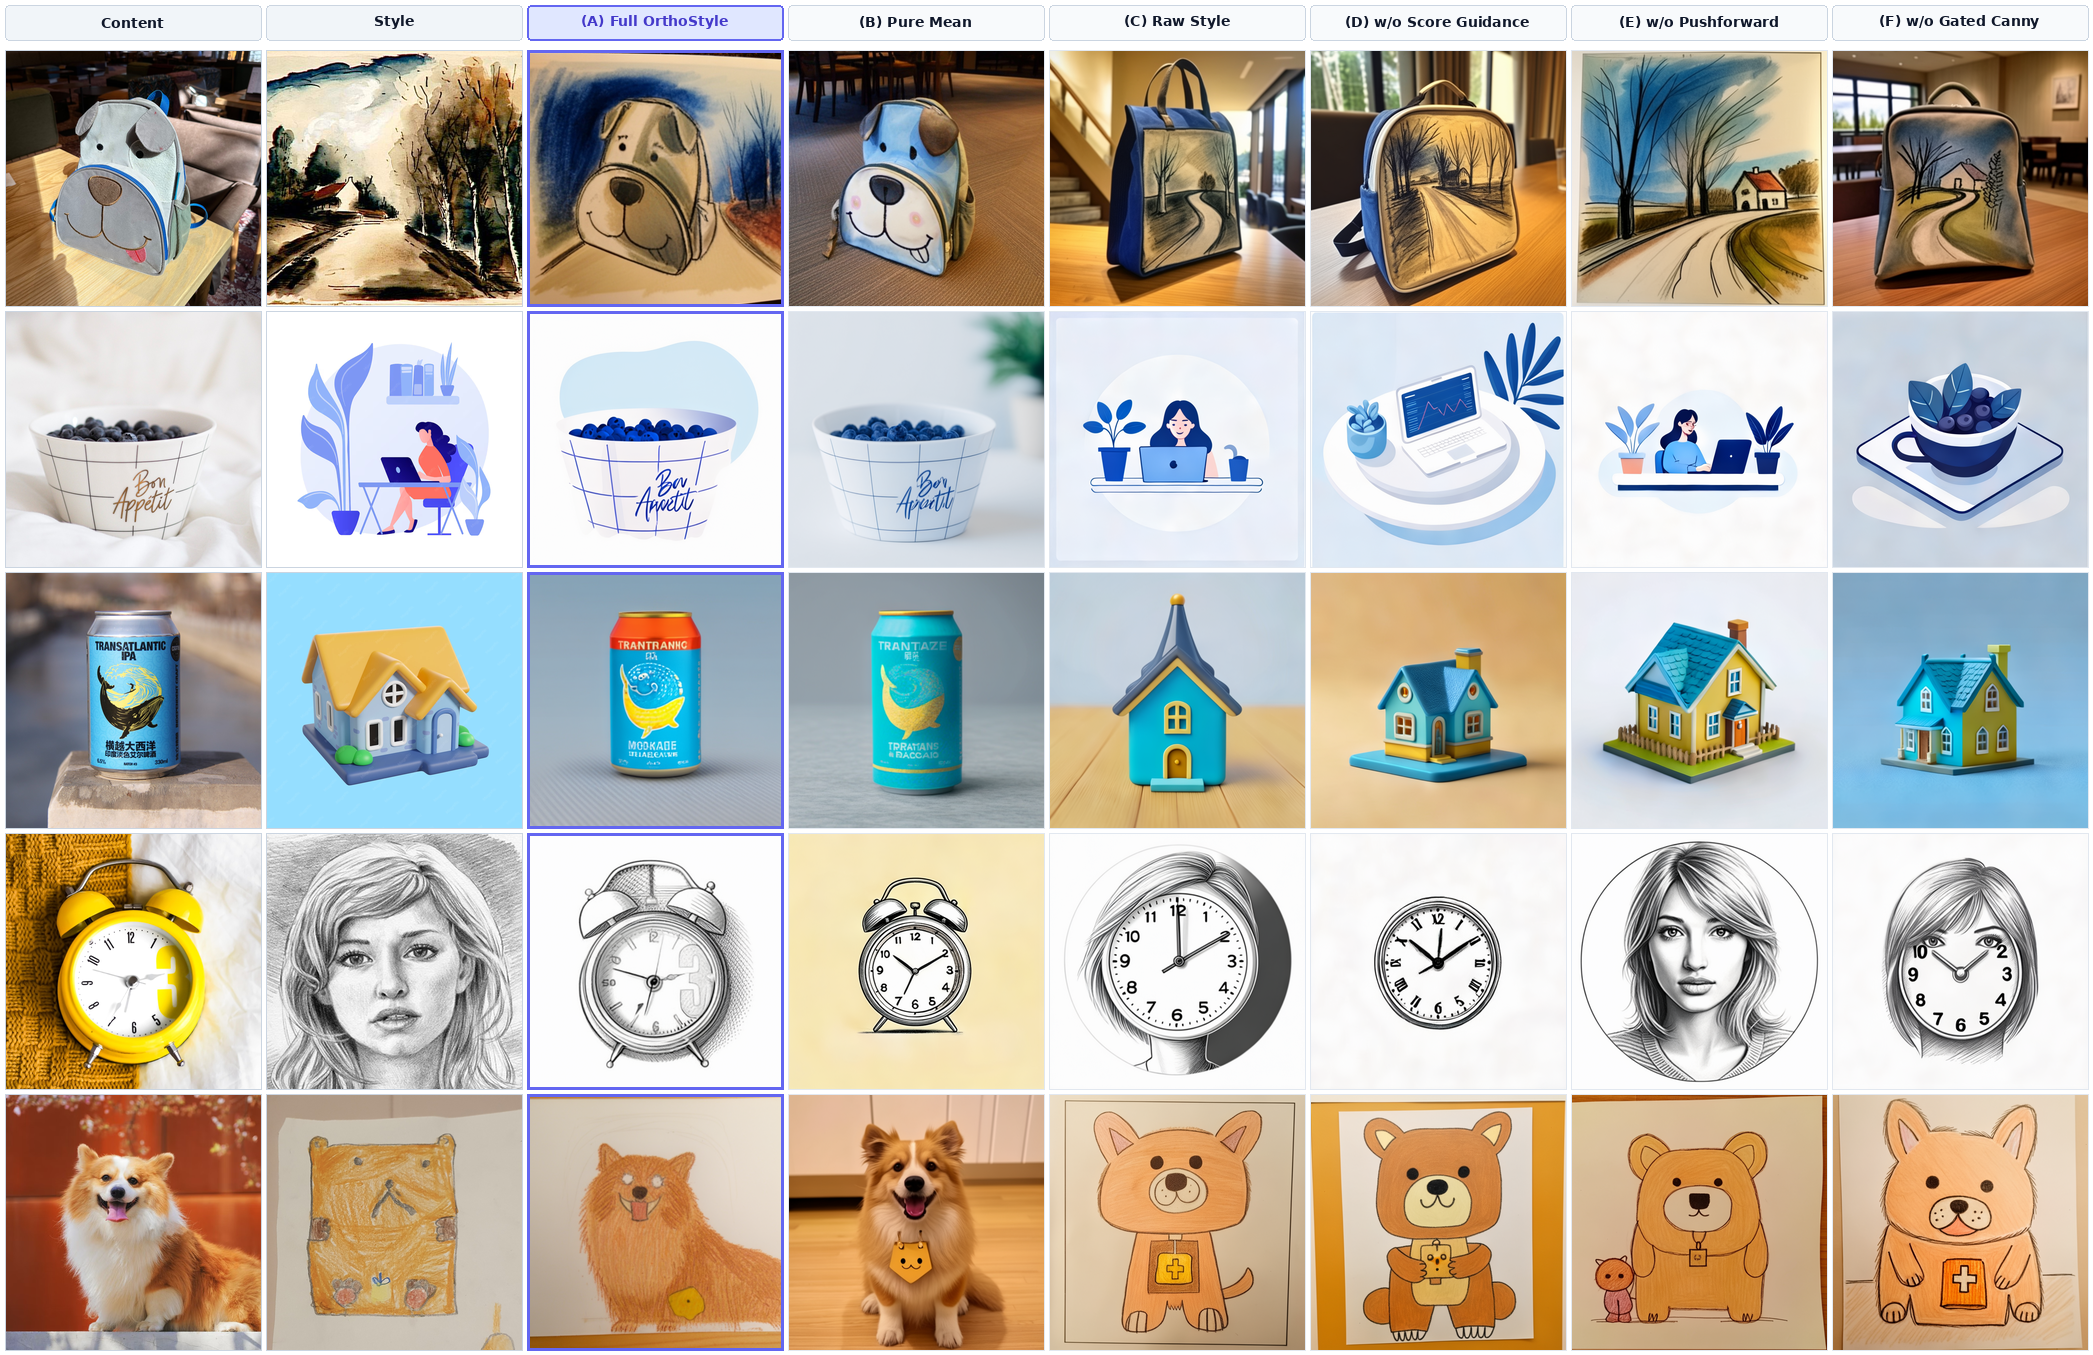
\includegraphics[width=\textwidth]{figs/ablation_components.png}
\caption{\textbf{Qualitative ablation of architectural components across diverse content-style matching pairs.} (A) Full \method provides balanced texture synthesis and silhouette preservation; (B) Pure mean pooling fails to transfer rich artistic stroke textures; (C) Raw style tokens allow foreign style objects to bleed into the subject; (D) Omitting score guidance degrades artistic vibrancy; (E) Removing early-step AdaIN pushforward severely disrupts global color distribution; (F) Disabling semantic edge gating introduces rigid background artifacts.}
\label{fig:ablation_components}
\end{figure*}

\begin{figure*}[t]
\centering
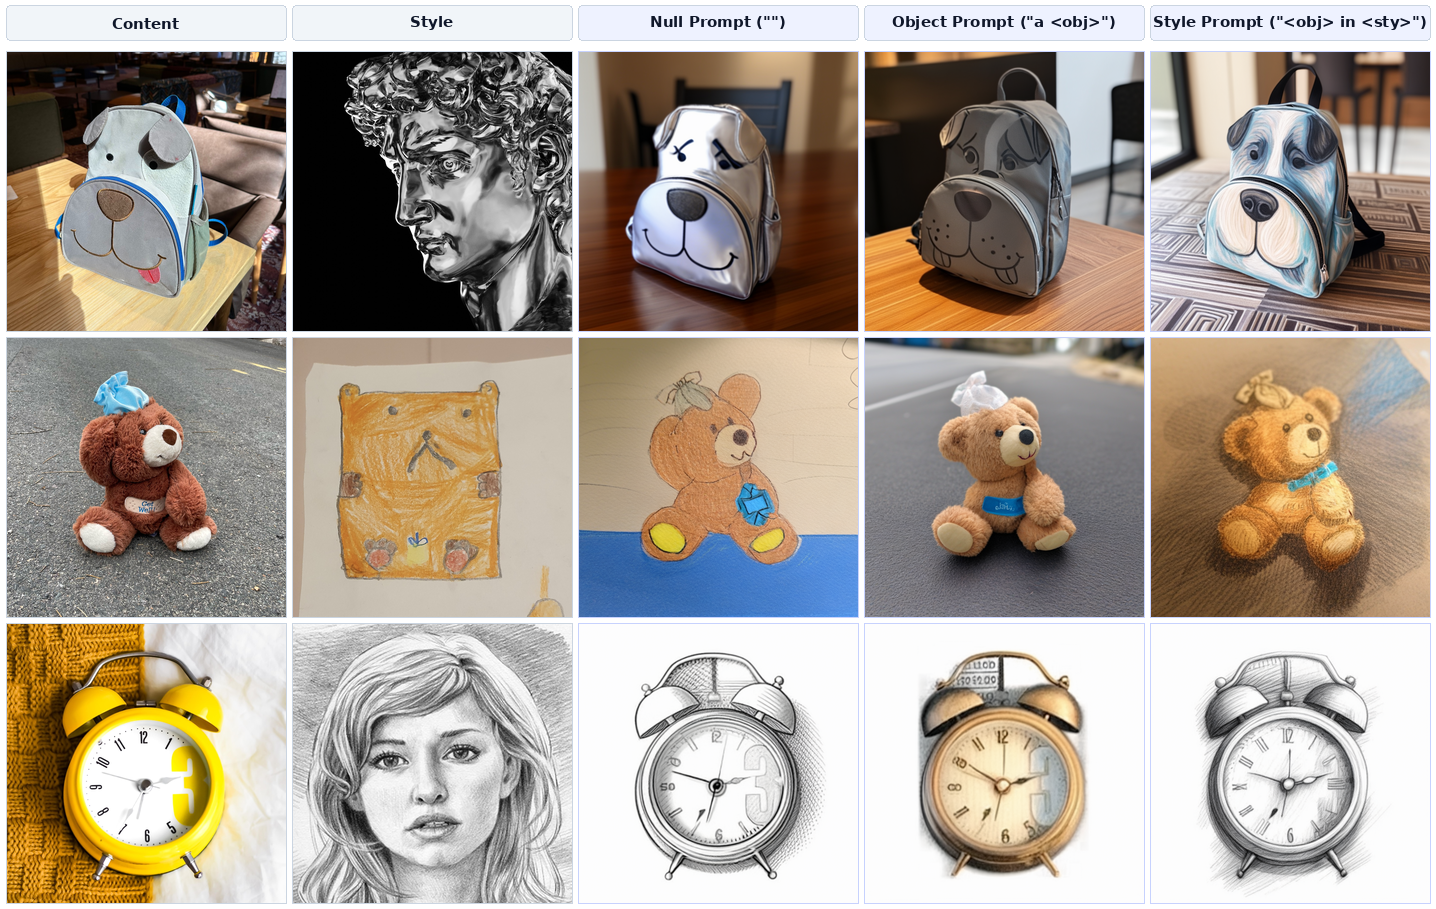
\includegraphics[width=0.95\textwidth]{figs/ablation_prompt_levels.png}
\caption{\textbf{Qualitative comparison across prompt conditioning levels.} Level 1 (Null prompt, \texttt{""}) relies purely on exemplar conditioning; Level 2 (Object prompt, \texttt{"a <obj>"}) reinforces target subject priors; Level 3 (Style prompt, \texttt{"<obj> in <sty> style"}) guides both subject identity and explicit artistic style keywords.}
\label{fig:ablation_prompts}
\end{figure*}
